% Foliensatz: "AFu-Kurs nach DJ4UF" von DK0TU, Amateurfunkgruppe der TU Berlin
% Lizenz: CC BY-NC-SA 3.0 de (http://creativecommons.org/licenses/by-nc-sa/3.0/de/)
% Autoren: Felix Baum <baum@campus.tu-berlin.de>
% Korrekturen: Sebastian Lange <dl7bst@dk0tu.de>

\documentclass[aspectratio=169]{beamer}

\usepackage[ngerman]{babel} % deutsche Worttrennung etc.
\usepackage[utf8]{inputenc} % UTF8 Text

\usepackage[super, comma, numbers, square, sort]{natbib}

\usepackage{hyperref}       % Hyperref Package für bessere Referenzen (todo)
\hypersetup{
	colorlinks=false,       %   false: boxed links; true: colored links
    %linkcolor=white,       %   color of internal links (change box color with linkbordercolor)
    citecolor=red,          %   color of links to bibliography
    filecolor=white,        %   color of file links
    urlcolor=blue           %   color of external links
}

\usepackage{multirow}
\usepackage{wasysym}  % Math Symbols like \permil
%\usepackage{colortbl}
%\usepackage{subscript}
%\usepackage{caption}
%\usepackage{setspace}
%\usepackage{xcolor}        % benutze CodeListe

% Footnote
%\usepackage{hanging}
%
%\setbeamertemplate{footnote}{%
%  \hangpara{2em}{1}%
%  \makebox[2em][l]{\insertfootnotemark}\footnotesize\insertfootnotetext\par%
%}


%\usepackage{pgf}
%\usepackage{tikz}
%\usetikzlibrary{arrows,automata}
%\usetikzlibrary{positioning}
%
%\tikzset{
%    state/.style={
%           rectangle,
%           rounded corners,
%           draw=black, very thick,
%           minimum height=2em,
%           minimum width=2pt,
%           inner sep=2pt,
%           text centered,
%           },
%}

%\usepackage{listings}
%\lstset{basicstyle=\small, numberstyle=\tiny, extendedchars=true, numbers=left, numbersep=5pt}
%\lstset{showtabs=false, showspaces=false, showstringspaces=false}
%%\lstset{backgroundcolor=\color{white!75!lightgray}, , frame=single}
%%\lstset{backgroundcolor=\color{white}}
%%\lstset{backgroundcolor=none}
%\lstset{keywordstyle=\color{blue!50!gray},  identifierstyle=\color{black}}
%\lstset{commentstyle=\color{green!50!gray}, stringstyle=\color{red!50!gray}}
%\lstset{language=C, fontadjust=true, tabsize=2, breaklines=true}
%\lstset{backgroundcolor=\color{white!75!lightgray}, caption=\lstname, frame=single}
%\lstset{emphstyle=\color{black}\fbox}
%
%% Keine "Listing:"-Caption
%\captionsetup{labelformat=empty,labelsep=none}
%
%% für mathematische Umgebungen
%\usepackage{amsmath,amsfonts,amssymb}
%
%\lstdefinestyle{Bash}{
%language=Bash,
%frame=single,
%rulecolor=\color{black},
%backgroundcolor=\color{gray!50},
%keywordstyle=\color{black},
%identifierstyle=,
%commentstyle=\color{black},
%stringstyle=\color{magenta!65!white},
%showstringspaces=false,
%basicstyle=\footnotesize\ttfamily\color{black},
%numbers=none,
%breaklines=true,
%captionpos=b
%}

%\usepackage{listings}
%
%\lstdefinestyle{basic}{
%    captionpos=t,%
%    basicstyle=\footnotesize\ttfamily,%
%    numberstyle=\tiny,%
%    numbers=left,%
%    stepnumber=1,%
%    frame=single,%
%    showspaces=false,%
%    showstringspaces=false,%
%    showtabs=false,%
%    %
%    keywordstyle=\color{blue},%
%    identifierstyle=,%
%    commentstyle=\color{gray},%
%    stringstyle=\color{magenta}%
%}



% fließende Boxen haben keinen Abstand
%\fboxsep0mm

% inkludiere Creative Commons Helper
%%%%%%%%%%%%%%%%%%%%%%%%%%%%%%%%%%%%%%%%%%%%%%%%%%%%%%%%%%%%%%%%
%% ccBeamer 0.1, 2007-07-02                                   %%
%% Written by Sebastian Pipping <webmaster@hartwork.org>      %%
%% ---------------------------------------------------------- %%
%% Licensed under Creative Commons Attribution-ShareAlike 3.0 %%
%% http://creativecommons.org/licenses/by-sa/3.0/             %%
%%%%%%%%%%%%%%%%%%%%%%%%%%%%%%%%%%%%%%%%%%%%%%%%%%%%%%%%%%%%%%%%


%% Images
\newcommand{\CcImageBy}[1]{%
	
\includegraphics[scale=#1]{texdata/creative_commons/cc_by_30.pdf}%
}
\newcommand{\CcImageCc}[1]{%
	
\includegraphics[scale=#1]{texdata/creative_commons/cc_cc_30.pdf}%
}
\newcommand{\CcImageDevNations}[1]{%
	
\includegraphics[scale=#1]{texdata/creative_commons/cc_dev_nations_30.pdf}%
}
\newcommand{\CcImageNc}[1]{%
	
\includegraphics[scale=#1]{texdata/creative_commons/cc_nc_30.pdf}%
}
\newcommand{\CcImageNd}[1]{%
	
\includegraphics[scale=#1]{texdata/creative_commons/cc_nd_30.pdf}%
}
\newcommand{\CcImagePd}[1]{%
	
\includegraphics[scale=#1]{texdata/creative_commons/cc_pd_30.pdf}%
}
\newcommand{\CcImageSa}[1]{%
	
\includegraphics[scale=#1]{texdata/creative_commons/cc_sa_30.pdf}%
}
\newcommand{\CcImageSampling}[1]{%
	
\includegraphics[scale=#1]{texdata/creative_commons/cc_sampling_30.pdf}%
}
\newcommand{\CcImageSamplingPlus}[1]{%
	
\includegraphics[scale=#1]{texdata/creative_commons/cc_sampling_plus_30.pdf}%
}


%% Groups
\newcommand{\CcGroupBy}[2]{% zoom, gap
	\CcImageCc{#1}\hspace*{#2}\CcImageBy{#1}%
}
\newcommand{\CcGroupByNc}[2]{% zoom, gap
	\CcImageCc{#1}\hspace*{#2}\CcImageBy{#1}\hspace*{#2}\CcImageNc{#1}%
}
\newcommand{\CcGroupByNcNd}[2]{% zoom, gap
	\CcImageCc{#1}\hspace*{#2}\CcImageBy{#1}\hspace*{#2}\CcImageNc{#1}\hspace*{#2}\CcImageNd{#1}%
}
\newcommand{\CcGroupByNcSa}[2]{% zoom, gap
	\CcImageCc{#1}\hspace*{#2}\CcImageBy{#1}\hspace*{#2}\CcImageNc{#1}\hspace*{#2}\CcImageSa{#1}%
}
\newcommand{\CcGroupByNd}[2]{% zoom, gap
	\CcImageCc{#1}\hspace*{#2}\CcImageBy{#1}\hspace*{#2}\CcImageNd{#1}%
}
\newcommand{\CcGroupBySa}[2]{% zoom, gap
	\CcImageCc{#1}\hspace*{#2}\CcImageBy{#1}\hspace*{#2}\CcImageSa{#1}%
}
\newcommand{\CcGroupDevNations}[2]{% zoom, gap
	\CcImageCc{#1}\hspace*{#2}\CcImageDevNations{#1}%
}
\newcommand{\CcGroupNcSampling}[2]{% zoom, gap
	\CcImageCc{#1}\hspace*{#2}\CcImageNc{#1}\hspace*{#2}\CcImageSampling{#1}%
}
\newcommand{\CcGroupPd}[1]{% zoom
	\CcImagePd{#1}%
}
\newcommand{\CcGroupSampling}[1]{% zoom
	\CcImageSampling{#1}%
}
\newcommand{\CcGroupSamplingPlus}[1]{% zoom
	\CcImageSamplingPlus{#1}%
}


%% Text
\newcommand{\CcLongnameBy}{Attribution}
\newcommand{\CcLongnameByNc}{Attribution-NonCommercial}
\newcommand{\CcLongnameByNcNd}{Attribution-NoDerivs}
\newcommand{\CcLongnameByNcSa}{Attribution-NonCommercial-ShareAlike}
\newcommand{\CcLongnameByNd}{Attribution-NoDerivs}
\newcommand{\CcLongnameBySa}{Attribution-ShareAlike}

\newcommand{\CcNote}[1]{% longname
	This work is licensed under the \textit{Creative Commons #1 3.0 License}.%
}


% generelles Thema auswählen
\usetheme{Goettingen} %Berlin spart ohne Sidebar allerdings angenehm Platz
% AnnArbor | Antibes | Bergen | Berkeley | Berlin | Boadilla | boxes | CambridgeUS | Copenhagen | Darmstadt | default | Dresden | Frankfurt | Goettingen | Hannover | Ilmenau | JuanLesPins | Luebeck | Madrid | Malmoe | Marburg | Montpellier | PaloAlto | Pittsburgh | Rochester | Singapore | Szeged | Warsaw

% Farben wählen
\usecolortheme{beetle}
% beaver | beetle | crane | default | dolphin | dove | fly | lily | orchid | rose | seagull | seahorse | sidebartab | structure | whale | wolverine

% Setze alle Farben auf Grau und Weiß
%\definecolor{craneorange}{RGB}{64,64,64}
%\definecolor{craneblue}{RGB}{255,255,255}

% Schriftart wählen
\usefonttheme{default}
% default | professionalfonts | serif | structurebold | structureitalicserif | structuresmallcapsserif

% Innere Themen(Kopf-, Fuß-, Sidebar usw)
%\useinnertheme{default}
\useinnertheme{circles}
% default | inmargin | rectangles | rounded | circles

% Äußere Themen (Anordnung der inneren, grenzen der Folien etc.)
\useoutertheme{infolines}
% default | infolines | miniframes | shadow | sidebar | smoothbars | smoothtree | split | tree

% Deaktiviere Navigations-Symbole ({} -> leer)
\setbeamertemplate{navigation symbols}{}
%\setbeamertemplate{navigation symbols}{\large \ifnum \insertframenumber <10 0\fi\insertframenumber/\inserttotalframenumber\vspace*{0.2ex}}

% Zeige ein Hintergrundbild
\setbeamertemplate{background canvas}{
        \hspace*{-2.0cm}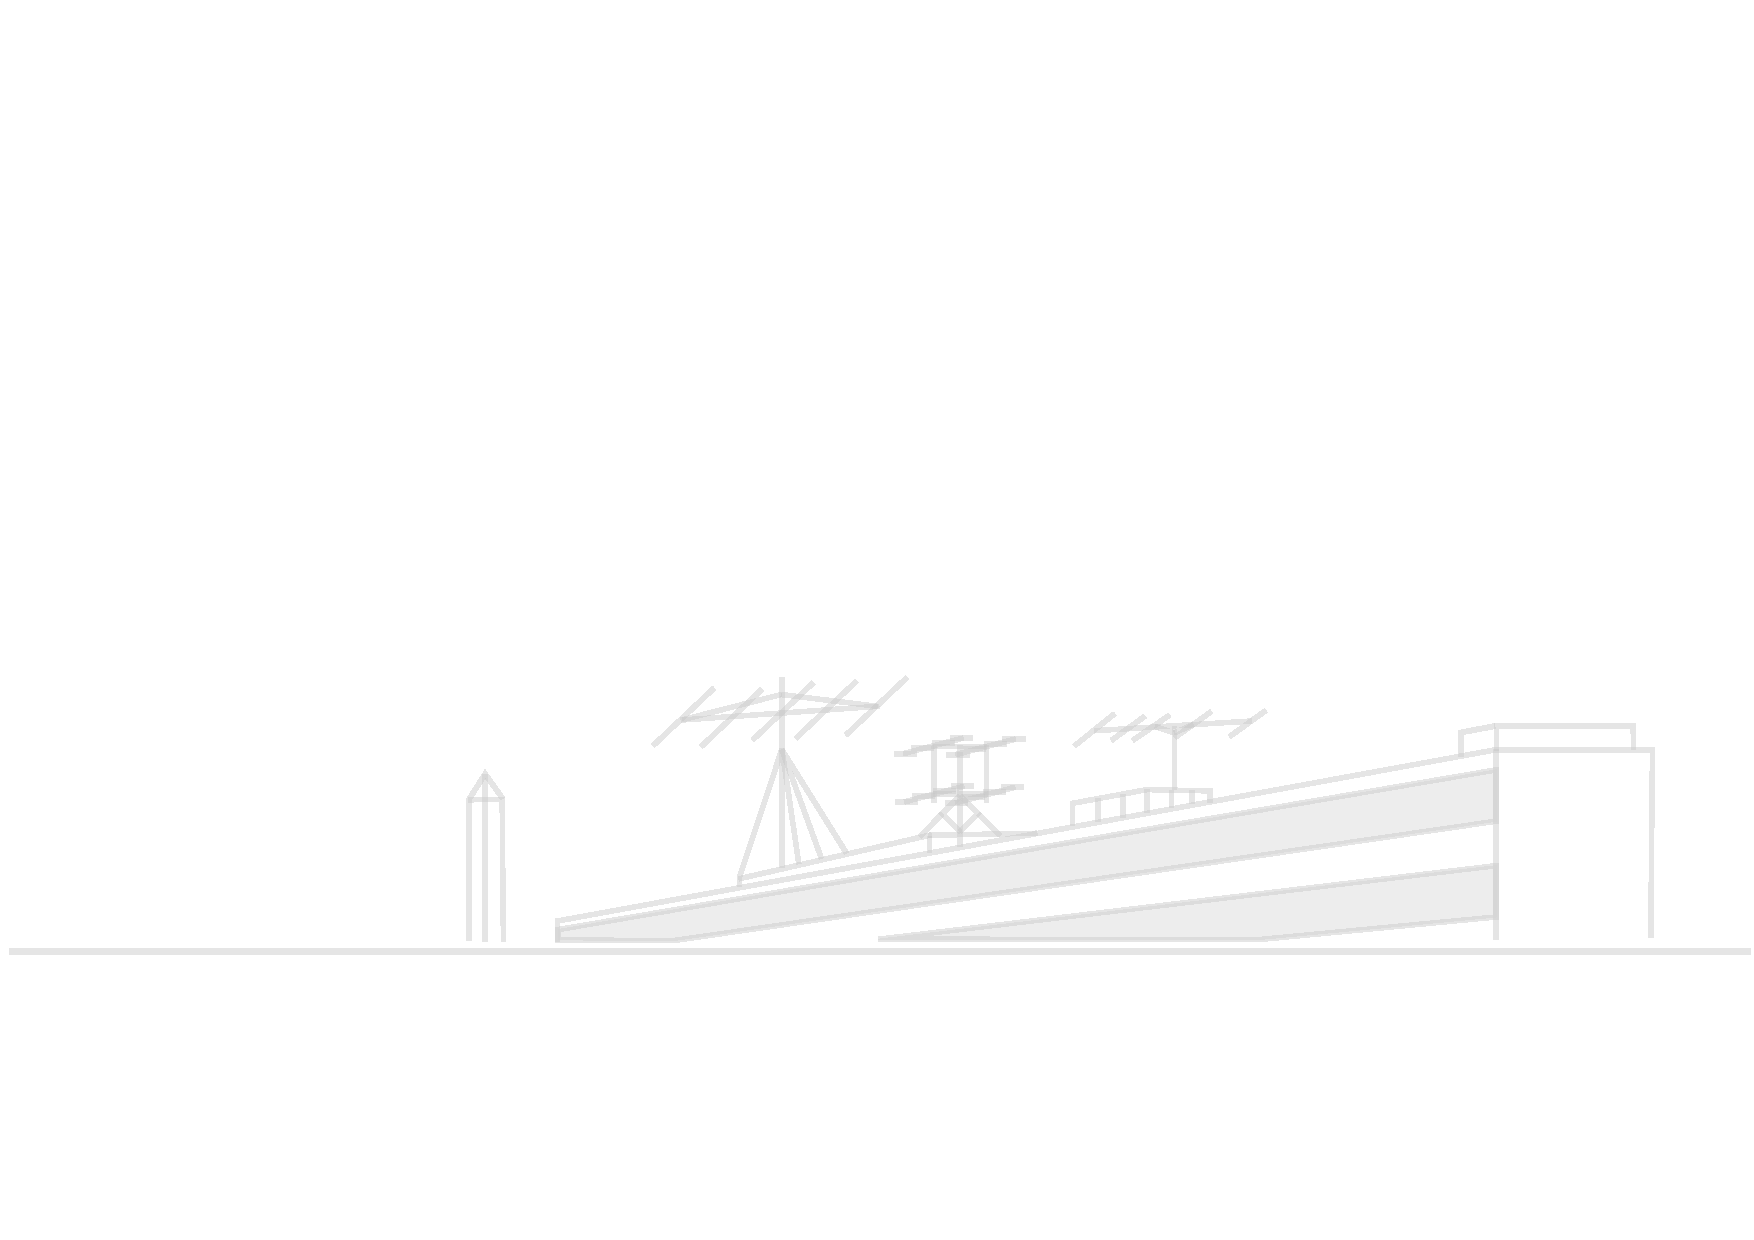
\includegraphics[width=17.8cm]{texdata/dk0tu_rooftop_background.pdf}
}

% Foliennummer einfügen
\setbeamertemplate{footline}[frame number]
%\setbeamertemplate{footline}{}

% Ändere das Zeichen vor jedem item
%\setbeamertemplate{itemize item}{\color{craneorange}$\blacktriangleright$}
%\setbeamertemplate{itemize subitem}{\color{craneorange}$\triangleright$}
%\setbeamertemplate{itemize subsubitem}{\color{craneorange}$\blacktriangleright$}

% Ändert die Blöcke 
\setbeamertemplate{blocks}[rounded][shadow=true]
% default | rounded [shadow=true|false]

%
% Eigene Kommandos
%

% Hack to get natbib and beamer working together. "The beamer user guide suggests
% that only the manual bibliography entry approach is supported"
% on some system it works out of the box, sometimes you need the hack :-(
% so check it --dl7bst
\ifdefined\newblock
    \relax
\else
    \newcommand{\newblock}{}
\fi

% \includedia command to generate png out of a dia file
% NEEDS installed dia and pdflatex option --shell-escape
\newcommand{\includedia}[1]{
    \immediate\write18{/usr/bin/dia #1.dia -e #1_diatmp.png -t png}
}

% RICHIG GROSSER FONT!
\newfont{\bigfont}{cmr10 at 144pt}
\newfont{\smallfont}{cmr10 at 8pt}

% Römische Ziffern
\makeatletter
\newcommand{\rmnum}[1]{\romannumeral #1}
\newcommand{\Rmnum}[1]{\expandafter\@slowromancap\romannumeral #1@}
\makeatother

% Schwarze Überschrift
%\setbeamercolor{frametitle}{fg=black}
%\setbeamercolor{title}{fg=black}

% Item- und Box-Farben
\definecolor{deepBlue}{HTML}{000066}
\setbeamercolor{itemize item}{fg=deepBlue}
\setbeamercolor{itemize subitem}{fg=deepBlue}
\setbeamercolor{description item}{fg=deepBlue}
\setbeamercolor{block title}{fg=deepBlue!100, bg=blue!15}
\setbeamercolor{block body}{fg=black, bg=blue!5}
\setbeamercolor{block title alerted}{fg=deepBlue, bg=red!75}
\setbeamercolor{block body alerted}{fg=black, bg=red!15}
\setbeamercolor*{block title example}{fg=blue!50, bg=blue!10}
\setbeamercolor*{block body example}{fg= blue, bg=blue!5}

%\setbeamercolor{section in head/foot}{parent=palette primary}
%\setbeamercolor{subsection in head/foot}{parent=palette secondary}
%\setbeamercolor{sidebar}{fg=darkblue,bg=yellow!90!orange}
%\setbeamercolor{title in sidebar}{fg=darkblue}
%\setbeamercolor{author in sidebar}{fg=darkblue}
%\setbeamercolor{section in sidebar}{fg=darkblue!10!black}
%\setbeamercolor{subsection in sidebar}{fg=darkblue!50!black}

% Titlepage Infos
\title{AFu-Kurs nach DJ4UF}
\author[DKØTU]{DKØTU\\ \footnotesize{Amateurfunkgruppe der TU Berlin}}
\institute[DKØTU]{\url{http://www.dk0tu.de} }

% PDF-Eigenschaften
\subject{DK0TU-Amateurfunkkurs nach DJ4UF}
\keywords{Amateurfunk Kurs HAM Radio Course CC-BY-NC-SA OpenSource TU Berlin DK0TU}

\subtitle{Technik 09: \\
           Die Wellenausbreitung \\[2em]}
\date{Stand 01.12.2016}
 \begin{document}

\begin{frame}
    \titlepage
    \vfill
    \begin{center}
        \ccbyncsaeu\\
        {\tiny This work is licensed under the \em{Creative Commons Attribution-NonCommercial-ShareAlike 3.0 License}.}\\[0.5ex]
         \tiny Amateurfunkgruppe der Technische Universität Berlin (AfuTUB), DKØTU
         %\includegraphics[scale=0.5]{img/DK0TU_Logo.pdf}
    \end{center}
\end{frame}


%fixme Referenzen/Fußnoten-Systematik vereinheitlichen

\section*{Einleitung}

\begin{frame}
    \frametitle{Wie kommen die Wellen um die Welt?}
    \begin{center}
       \begin{figure}
          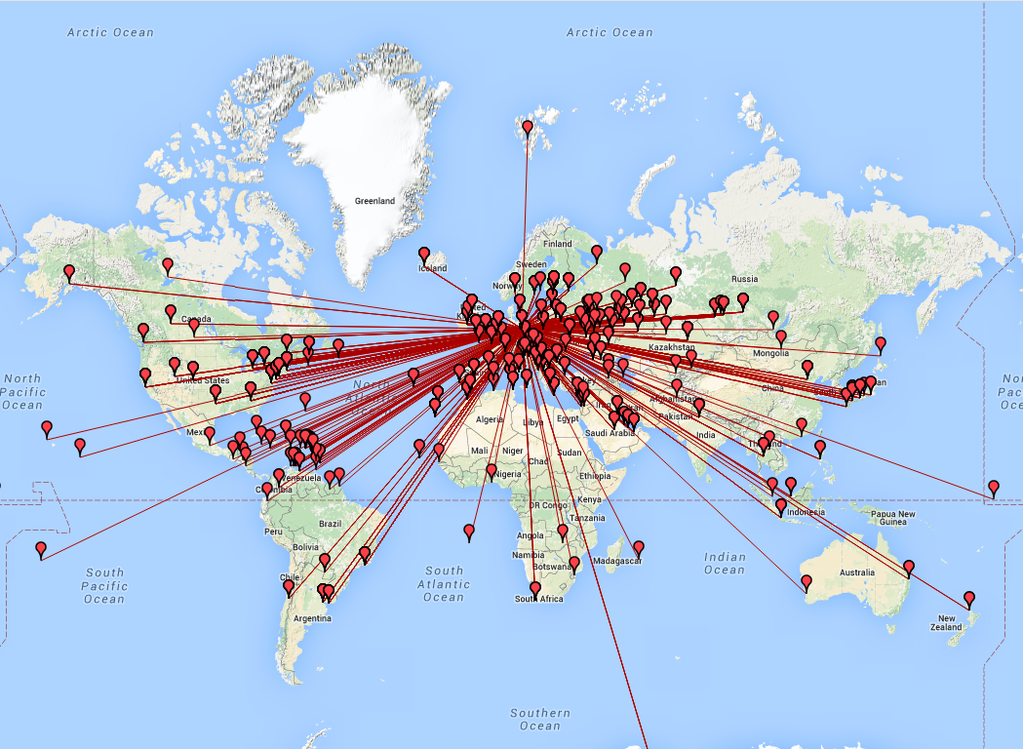
\includegraphics[width=1\textwidth,height=.75\textheight,keepaspectratio]{e09/cqww-kontakte-2015.png}
          \caption{Funkkontakte beim CQWW-SSB 2015 von DK\O TU}
       \end{figure}
    \end{center}
\end{frame}

\begin{frame}
  \frametitle{Raum und Bodenwelle}
    \begin{center}
      \begin{figure}
         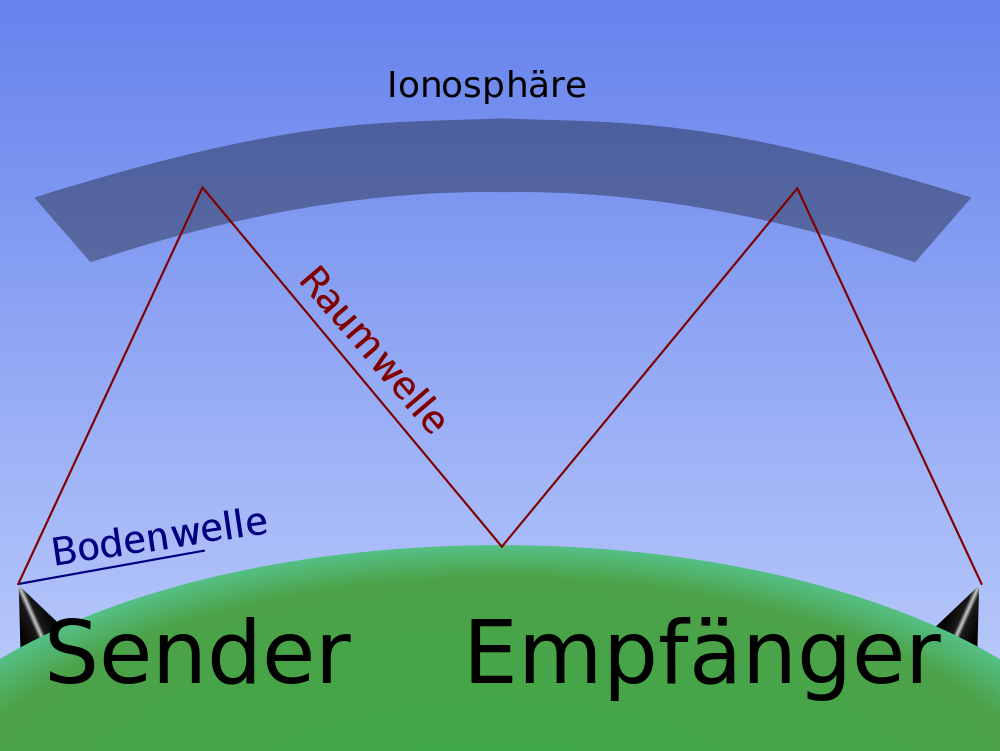
\includegraphics[width=1\textwidth,height=.75\textheight,keepaspectratio]{e09/Ionospheric_reflectionpng.png}
         \attribcaption{Reflektion an der Ionosphäre}{Sebastian Janke}{https://commons.wikimedia.org/wiki/File:Ionospheric_reflection-de.svg}{\ccbysa}
       \end{figure}
    \end{center}
\end{frame}

\begin{frame}
    \frametitle{Boden- und Raumwelle}
    \textbf{Bodenwelle}
    \begin{itemize}
	    \item Folgt der Erdkrümmung
	    \item Stark vorhanden bei Langwelle und Mittelwelle
	    \item Viele Verluste durch Berge, Wälder und Städte
    \end{itemize}
    \textbf{Raumwelle}
    \begin{itemize}
	    \item Meist genutzt bei Kurzwelle (manchmal auch UHF, VHF)
	    \item Reflektion an der Ionosphäre 
	    \item Nicht zuverlässig für Überreichweiten
    \end{itemize}
\end{frame}

\section*{Bodenwelle}
\begin{frame}
    \frametitle{Bodenwelle}
    \begin{itemize}
      \item Bei LF über $400km$
      \item $80m$ Wellenlänge ($3.5MHz$) $\rightarrow~\thicksim150km$ Reichweite
      \item $10m$ Wellenlänge ($28MHz$) $\rightarrow~\thicksim30km$ Reichweite
      \item Reichweite hängt auch stark vom Untergrund ab
    \end{itemize}
\end{frame}

\section*{Raumwelle}
    
\begin{frame}
    \frametitle{Raumwelle}
    \begin{center}
      \begin{figure}
        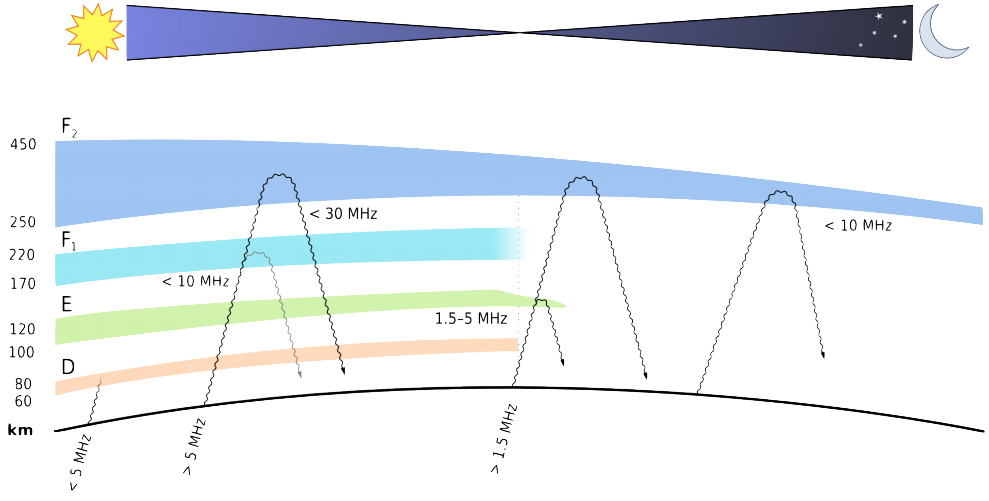
\includegraphics[width=\textwidth,height=.75\textheight,keepaspectratio]{e09/schichten_behelf_43.png}
        \caption{Amateurfunkbehelf S.43 \ExternalLink \url{http://ham.granjow.net/builds/Amateurfunkbehelf.pdf}}
      \end{figure}
    \end{center}
\end{frame}

\begin{frame}
    \frametitle{Sonnenflecken-Zyklus}
    \begin{itemize}
    			\item Bei Sonneneinstrahlung werden Moleküle in der Ionosphäre durch EUV-Strahlung ionisiert
			\item Maximum ungefähr alle 11 Jahre
                        \item HF Frequenzen ab $\thicksim20MHz$ sind bei einem Minimum nicht verwendbar
       		 	\item Bei einem Maximum quasi täglich DX-Verbindungen mit weniger als $10W$ machbar 
        		\item Nächstes Maximum vermutlich 2022
    \end{itemize}
	\begin{center}
         \begin{figure}
      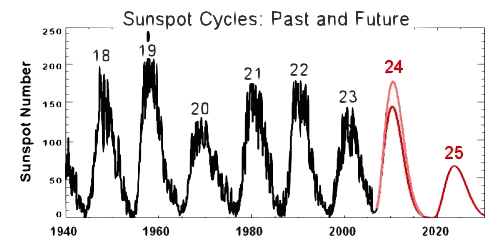
\includegraphics[width=.8\textwidth,height=.3\textheight,keepaspectratio]{e09/Predictions_sunspot.png}
      \attribcaption{Sonnenflecken Vorhersage}{Scientific data, based on prediction by David Hathaway}{https://commons.wikimedia.org/wiki/File_3APredictions3_strip.jpg}{\ccpd}
    \end{figure}
    \end{center}
\end{frame}

\begin{frame}
    \frametitle{D-Schicht}
    \begin{itemize}
    			\item Tagsüber und verschwindet nach Sonnenuntergang sehr schnell
			\item Dämpft Frequenzen unter $5MHz$ (160m und 80m unbenutzbar)
                        \item HF Frequenzen ab $\thicksim20MHz$ sind bei einem Minimum nicht verwendbar
       		 	\item Bei hoher Sonnenaktivität Möbel-Dellinger-Effekt (Kurzzeitig ganzes KW-Band unbenutzbar)
    \end{itemize}
    \begin{center}
       \begin{figure}
      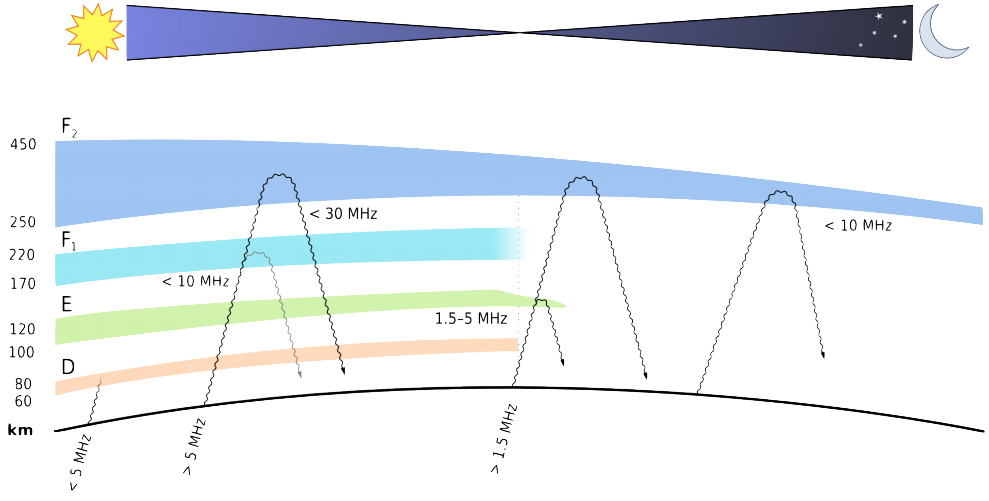
\includegraphics[width=.6\textwidth,height=.4\textheight,keepaspectratio]{e09/schichten_behelf_43.png}
      \caption{Amateurfunkbehelf s.43 \ExternalLink \url{http://ham.granjow.net/builds/Amateurfunkbehelf.pdf}}
    \end{figure}
    \end{center}
\end{frame}

\begin{frame}
    \frametitle{E-Schicht}
    \begin{itemize}
    		\item Manchmal Tagsüber
			\item Reflektiert HF-Bänder 10m, 6m
            \item Reflektiert gelegentlich 2m (Sporadic-E) \footnote{\tiny \url{http://www.dk0tu.de/blog/2012/11/27_Sporadic-E_QSO_mit_Spanien/}}
            \item mit sehr starken Signalen zwischen 750km und 2200 km (Short-Skip)
    \end{itemize}
    \begin{center}
      \begin{figure}
        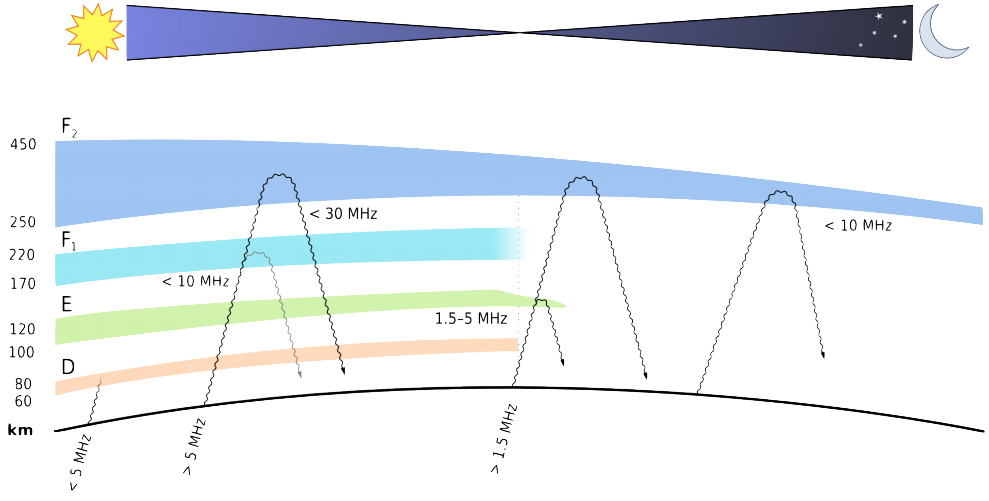
\includegraphics[width=.8\textwidth,height=.4\textheight,keepaspectratio]{e09/schichten_behelf_43.png}
       \caption{Amateurfunkbehelf s.43 \ExternalLink \url{http://ham.granjow.net/builds/Amateurfunkbehelf.pdf}}
      \end{figure}
    \end{center}
\end{frame}

\begin{frame}
    \frametitle{F-Schichten}
    \begin{itemize}
        \item $F_1$- und $F_2$-Schicht
        \item $F_2$-Schicht besteht auch nachts (langsame Rekombination)
        \item Für KW wichtig, da beständige Schichten
        \item mit sehr starken Signalen zwischen 750km und 2200 km (Short-Skip)
    \end{itemize}
	\begin{center}
          \begin{figure}
            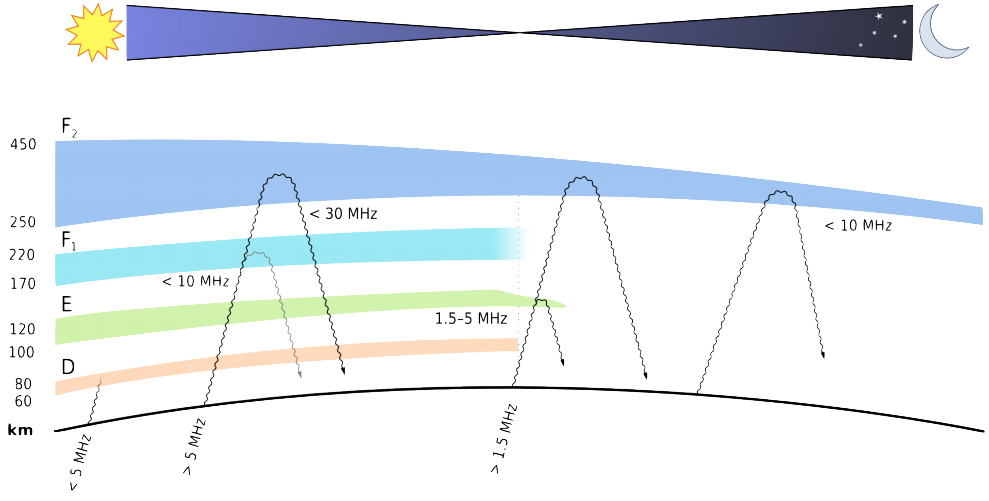
\includegraphics[width=.8\textwidth,height=.4\textheight,keepaspectratio]{e09/schichten_behelf_43.png}
              \caption{Amateurfunkbehelf s.43 \ExternalLink \url{http://ham.granjow.net/builds/Amateurfunkbehelf.pdf}}
          \end{figure}
    \end{center}
\end{frame}

\section*{DX-Propergation}

\begin{frame}
  \frametitle{Einige Einflüsse auf die Ionosphere}
  \begin{center}
  \begin{figure}
    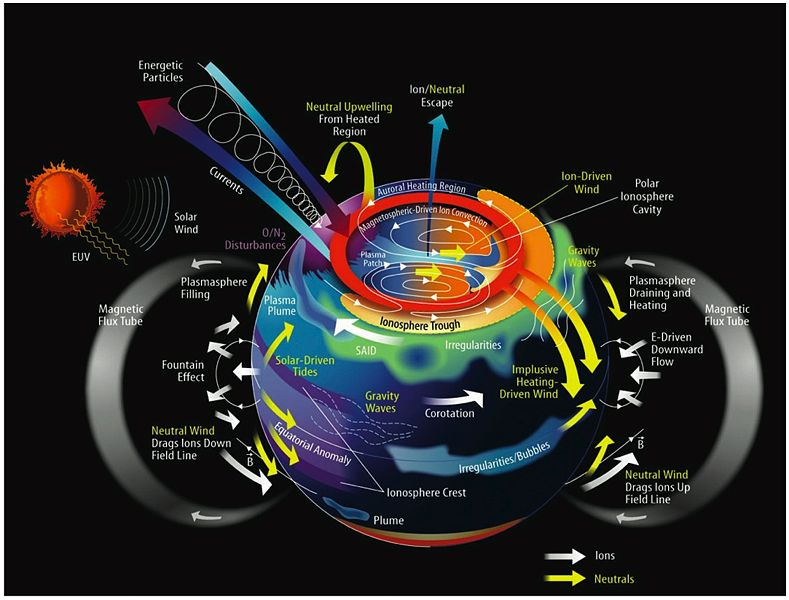
\includegraphics[width=.8\textwidth,height=.8\textheight,keepaspectratio]{e09/Ionosphere-Thermosphere_Processes.jpg}
    \attribcaption{Thermische Einflüsse auf die Ionosphäre}{NASA}{https://commons.wikimedia.org/wiki/File:Ionosphere-Thermosphere_Processes.jpg}{\ccpd}
    \end{figure}
  \end{center}
\end{frame}

\begin{frame}
    \frametitle{Aurora}
	\begin{center}
        \begin{block}{DX-Propergation}
        \item Einige Seiten bieten eine Vorschau oder aktuelle Infos über die Ausbreitungsbedingungen.
        \item \url{http://www.dr1a.com/pages/en/dx-propagation.php}
        \item \url{https://dxheat.com/dxc/}
        \item \url{https://www.youtube.com/watch?v=TQkzzJqMA3g}
        \end{block}
    \end{center}
\end{frame}

\section*{Besonderes}

\begin{frame}
    \frametitle{Sonstiges}
    \begin{description}
      \item[MUF] maximum usable frequency bei welcher die Wellen noch reflektiert werden
      \item[Tote Zone] Bereich, bei dem ein Signal nicht zu hören ist, da keine Welle dort niederschlägt
      \item[Fading] Schicht baut sich ab und das Signal schwindet oder destruktive Interferenz von Raum und Bodenwelle
      \item[Grey Line] Zone des Sonnenauf- und -untergangs mit besonderen Ausbreitungsbedingungen
    \end{description}
\end{frame}

\begin{frame}
  \frametitle{Fading bei Sonnensturm}
  \begin{center}
    \begin{figure}
    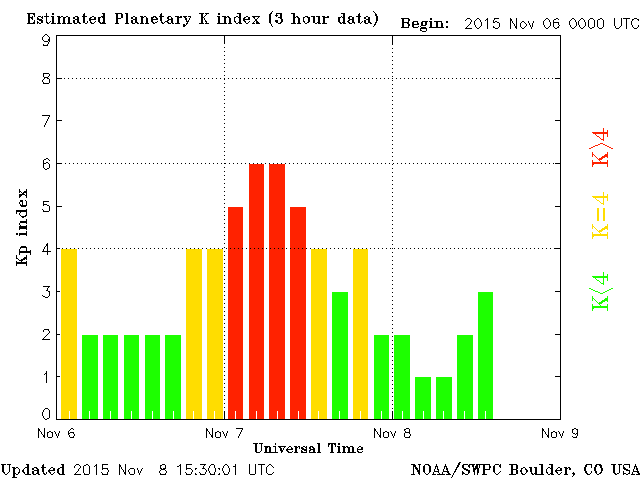
\includegraphics[width=.8\textwidth,height=.55\textheight,keepaspectratio]{e09/planetary-k-index.png}
    \caption{Space Weather Prediction Center \ExternalLink \url{http://www.swpc.noaa.gov/impacts/hf-radio-communications}}
    \end{figure}
    \begin{itemize}
    \item Planetary K-Index gibt Stärke des Sonnensturms an. 
    \item Beim Funken in JT65/JT9 auf 20m verschwand das Signal binnen einer Minute im Wasserfall und war danach komplett tot.
    \end{itemize}
  \end{center}
\end{frame}

\begin{frame}
    \frametitle{Aurora}
	\begin{center}
        \begin{figure}
      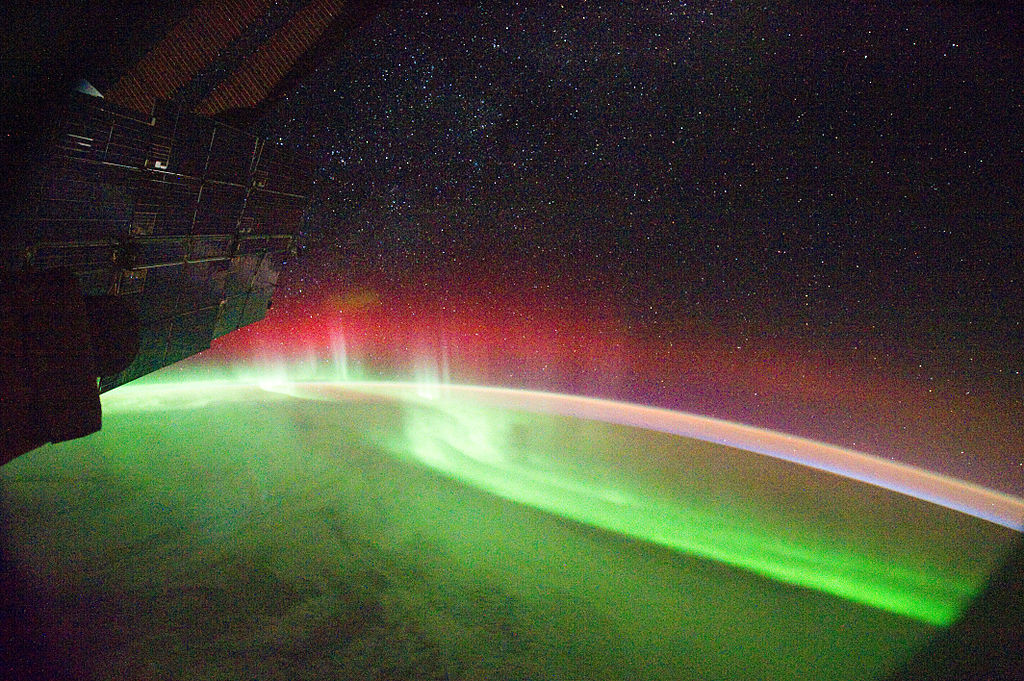
\includegraphics[width=.9\textwidth,height=.75\textheight,keepaspectratio]{e09/Aurora_Seen_From_Space_by_NASA.jpg}
      \attribcaption{Aurora vom Weltall aus}{NASA}{https://commons.wikimedia.org/wiki/File:Aurora_Seen_From_Space_by_NASA.jpg}{\ccpd}
    \end{figure}
    \end{center}
\end{frame}

\begin{frame}
    \frametitle{Troposphärische Überreichweiten}
    \begin{itemize}
      \item Beugt UKW (dadurch Überreichweite)
      \item bekannt als Tropo da nicht Ionosphäre sondern Troposphäre (15km Höhe)
      \item Kalte Luft unten, warme Luft oben sorgt für Brechung der UKW Wellen
      \item Entfernungen bis ca 700km
    \end{itemize}
    	\begin{center}
        \begin{figure}
      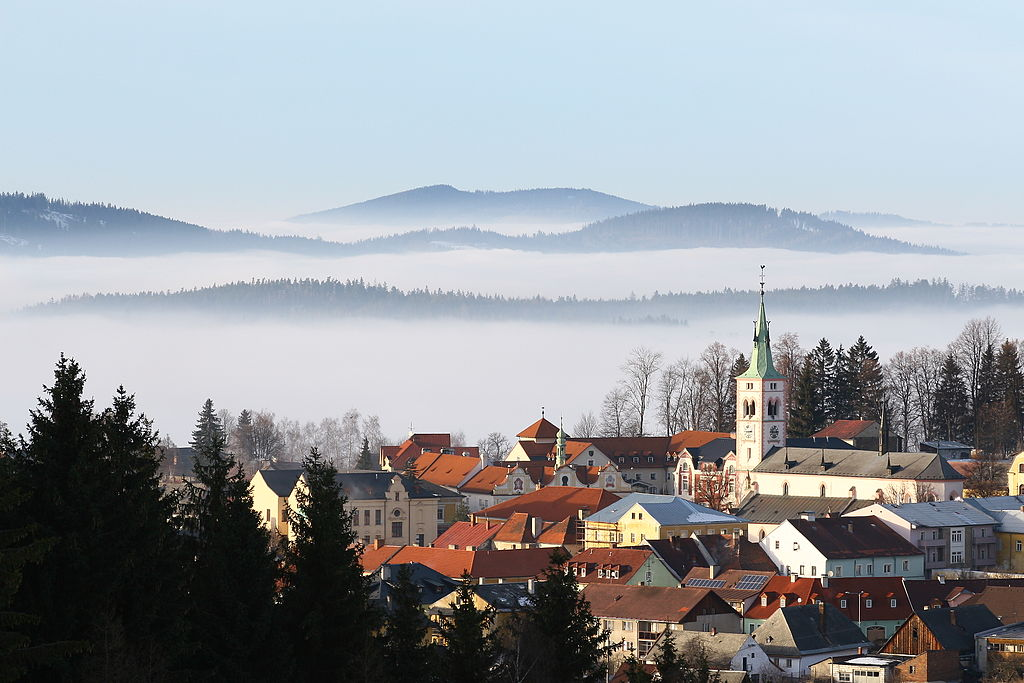
\includegraphics[width=.65\textwidth,height=.5\textheight,keepaspectratio]{e09/tropo.jpg}
      \attribcaption{Inversionswetterlage}{Adam Hauner}{https://commons.wikimedia.org/wiki/File:Kašperské Hory od Liščího vrchu.jpg}{\ccby}
    \end{figure}
    \end{center}
\end{frame}

%\begin{frame}
%    \frametitle{Prüfungsfrage}

%    \begin{center}
%    \begin{tabular}{l||p{.8\textwidth}}\hline
%      \textbf{TI101} & \textbf{Welche ionosphärischen Schichten bestimmen die Wellenausbreitung am Tage?} \\\hline\hline
%         A 	  & Die E- und D-Schicht \\\hline
%         B 	  & Die F\textsubscript{1}- und F\textsubscript{2}-Schicht \\\hline
%         C	  & Die E- und F-Schicht \\\hline
%         D \only<2>\checkmark 	  & Die D-, E-, F\textsubscript{1}- und F\textsubscript{2}-Schicht\\\hline
%    \end{tabular}
% 	\end{center}
%\end{frame}
%
%\begin{frame}
%    \frametitle{Prüfungsfrage}

%   \begin{center}
%   \begin{tabular}{l||p{.8\textwidth}}\hline
%      \textbf{TI102} & \textbf{Welche ionosphärischen Schichten bestimmen die Wellenausbreitung in der Nacht?} \\\hline\hline
%         A 	  & Die D-, E- und F\textsubscript{2}-Schicht \\\hline
%         B \only<2>\checkmark 	  & Die F\textsubscript{2}-Schicht \\\hline
%         C	  & Die F\textsubscript{1}- und F\textsubscript{2}-Schicht \\\hline
%         D 	  & Die D- und E-Schicht\\\hline
%    \end{tabular}
% 	\end{center}
%\end{frame}



\section*{Referenzen}

\begin{frame}
    \frametitle{Referenzen/Links}
    
    \footnotesize
    \begin{itemize}
        \item Moltrecht E 09: \\
              \url{http://www.dj4uf.de/lehrg/e09/e09.html}
        \item Aurora (Youtube): \\
              \url{https://www.youtube.com/watch?v=izYiDDt6d8s}
        \item Spradic E QSO \\
              \url{http://www.dk0tu.de/blog/2012/11/27_Sporadic-E_QSO_mit_Spanien/}
	\item Space Weather Prediction Center -- HF Radio Communications \\
	      \url{http://www.swpc.noaa.gov/impacts/hf-radio-communications}
    \end{itemize}

\end{frame}

% Hier könnte noch eine Kontaktfolie stehen

\end{document}

